\chapter{ Servlet编程}
\label{chp:JavaEE-servlet-programming}

\section*{基本信息}
\sline
\begin{description}
\item[课程名称:] Java应用与开发
\item[授课教师:] 王晓东
\item[授课时间:] 第九周
\item[参考教材:] 本课程参考教材及资料如下:
  \begin{itemize}
  \item 吕海东,张坤 编著,Java EE企业级应用开发实例教程,清华大学出版社,2010年8月
  \end{itemize}
\end{description}

\section*{教学目标}

\sline

\begin{enumerate}
\item 理解Web的概念及工作模式,掌握Java Web应用的构成。
\item 掌握Servlet的概念、体系结构及生命周期管理基本原理。
\item 掌握Servlet的编程及配置方法,了解Servlet的在Tomcat服务器上的部署方式(war)。
\end{enumerate}  

\section*{授课方式}

\sline
\begin{description}
\item[理论课:] 多媒体教学、程序演示
\item[实验课:] 上机编程
\end{description}

\newpage
\section*{教学内容}
\sline

%%%%%%%%%%%%%%%%%%%%%%%%%%%%%%%%%%%%%%%%%%%%%%%%%%%%%%%%%%%%%%%%%

JSP和JSF都是建立在Servlet基础之上的,其他Web框架
如Struts、WebWork和Spring MVC都是基于Servlet。所有很有必要对Servlet编程
技术进行更为深入的研究,这是我们未来学习框架技术和形成自己框架软件的基
础。


\section{Web基础}

\subsection{什么是Web}

\begin{itemize}
\item Web本质上就是Internet上所有文档(资源)的集合,如HTML网
  页、CSS、JS、图片、动态网页、声音、视频等。
\item Web文档保存在Web站点上,Web站点驻留在Web服务器上。
\item 常见Web服务器
  有Apache、IIS、WebLogic、GlassFish、JBoss和Tomcat等。
\end{itemize}
Web文档都有唯一的地址,通过URL来进行定位:

{\Blue\kai 协议://IP地址:端口/站点名/目录/文件名}

\begin{javaCode}
  http://210.30.108.30:8080/jycrm/admin/login.jsp
  ftp://210.30.108.30/software/jdk.zip
\end{javaCode}

\subsection{Web工作模式} 

Web使用请求/响应模式进行工作,Web服务器不会主动将Web文档发送到客户端。

\begin{enumerate}\kai
\item 由客户(一般是浏览器)使用URL对Web文档进行请求;
\item Web服务器接收并处理请求;
\item 处理结束后将响应内容发送到客户。
\end{enumerate}

\begin{itemize}
\item Web请求方式主要有{\Red GET、POST}、PUT、DELETE和HEAD。
\item Web响应一般情况下是HTML文档,也可以是其他类型资源。
\item Web使用MIME (Multipurpose Internet mail Extensions)标准来确定具
  体的响应类型。HTTP响应总体上分为两类:文本类型(纯文本字
  符、HTML、XML)和二进制原始类型(图片、声音、视频)。
\end{itemize}

\subsection{Java Web应用的构成}

\begin{itemize}
\item HTML文档
\item CSS
\item JavaScript
\item 图片文件
\item Servlet
\item JSP
\item JavaBean类
\item Java Lib
\item Web配置文件:/WEB-INF/web.xml
\end{itemize}

\notice{演示} 在Eclipse中创建一个Java Dynamic Project。

\section{Servlet概述}

\subsection{Servlet概述}

\subsubsection{什么是Servlet} 

\begin{itemize}
\item Servlet是一种Java Class,它运行在Java EE的Web容器内,由Web容器负责它的对象的创建和销毁,不能直接由其它类对象来调用。
\item 当Web容器接收到对它的HTTP请求时,自动创建Servlet对象,并自动调用它的doPost或doGet方法。
\end{itemize}

\subsubsection{Servlet的主要功能}

\begin{itemize}
\item 接收用户HTTP请求。
\item 取得HTTP请求提交的数据。
\item 调用JavaBean对象的方法。
\item 生成HTML类型或非HTML类型的HTTP动态响应。
\item 实现其他Web组件的跳转,包括重定向和转发。
\end{itemize}


\subsubsection{与Servlet相近的技术}

\begin{itemize}
\item CGI (Common Gateway Interface)。
\item MS的HTTP DLL技术。
\item Perl语言编写的处理代码。
\end{itemize}

\subsubsection{Servlet的特点}

\begin{itemize}
\item 使用Java语言编写。
\item 可以运行在符合J2EE规范的所有应用服务器上,实现跨平台运行。
\item 单进程、多线程技术,运行速度快,节省服务器资源。
\end{itemize}

\subsection{Servlet体系结构}

\begin{itemize}
\item javax.servlet包含支持所有协议的的通用的Web组件接口和类;
\item javax.servlet.http包含了支持HTTP协议的接口和类。
\end{itemize}

\begin{figure}[htb]
\centering
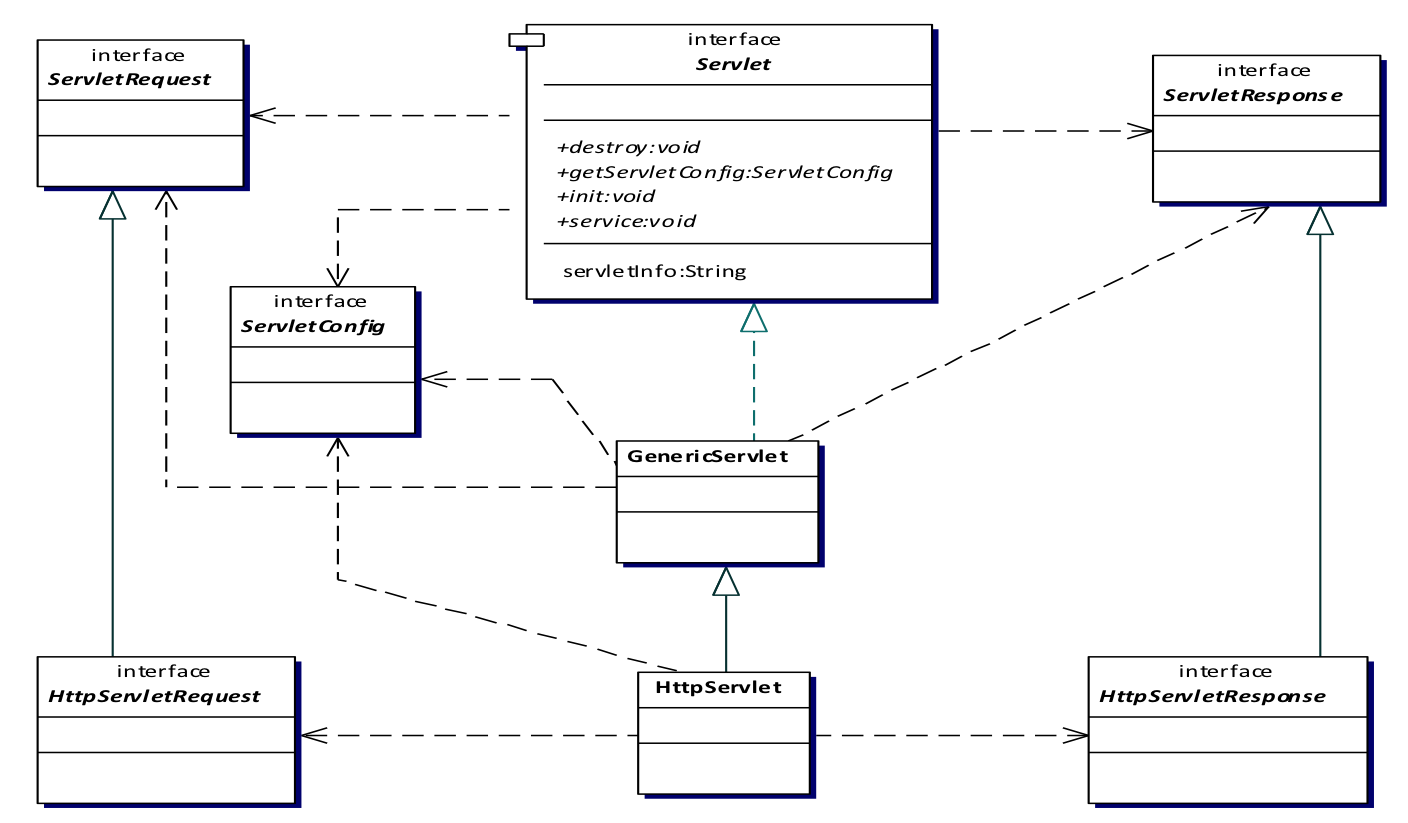
\includegraphics[width=0.8\textwidth]{images/JavaEE-servlet-programming/fig-sevlet-class-map.png}
\caption{Servlet类结构}
\label{fig:sevlet-class-map}
\end{figure}

\section{Servlet编程}

\subsection{引入包} 

\begin{javaCode}
  import java.io.*;
  import javax.servlet.*;
  import javax.servlet.http.*;
\end{javaCode}

\subsection{类定义} 

编写接收HTTP请求并进行HTTP响应的Servlet需要继承javax.servlet.http.HttpServlet。

\begin{javaCode}
public class LoginAction extends HttpServlet {
  // Code goes on.
}
\end{javaCode}

\subsection{重写doGet方法} 

父类HttpServlet的doGet方法是空的,没有实现任何代码,子类需要重写此方法。

\begin{javaCode}

public void doGet(HttpServletRequest request, HttpServletResponse response) 
throws ServletException, IOException {
  // Rewrite the method.
}
\end{javaCode}

当HTTP请求为GET时自动运行,每次请求都运行一次。

\subsection{重写doPost方法} 

编写Servlet需要重写父类的doPost方法。

\begin{javaCode}
public void doPost(HttpServletRequest request, HttpServletResponse response)  
throws ServletException, IOException {
  // Rewrite the method.
}
\end{javaCode}

当请求方式为POST时自动运行,每次请求都运行一次。

{\hei\Red doGet和doPost方法都接收Web容器自动创建的请求对象和响应对象,使得Servlet能够解析请求数据和发送响应给客户端。}

\subsection{重写init方法} 

当Web服务器创建Servlet对象后,会自动调用init方法完成初始化功能,一般将耗时的连接数据库和打开外部资源文件的操作放在init方法中。

init方法在Web容器创建Servlet对象后立即执行,且只执行一次。

\begin{javaCode}
  public void init(ServletConfig config) throws ServletException {
    super.init(config);
    // 这里放置初始化工作代码.
  }
\end{javaCode}

{\kai 在init方法中使用Web容器传递的config对象取得Servlet的各种配置初始参数,进而使用这些参数完成读取数据库或其他外部资源。}

\subsection{重写destroy方法} 

当Web容器需要销毁Servlet对象时,一般是Web容器停止运行或Servlet源代码修改而重新部署时,Web容器自动运行destroy方法完成清理工作,如关闭数据库连接和I/O流。

\begin{javaCode}
  public  void destroy() {
    try {
      cn.close();
    } catch (Exception e) {
      application.Log("登录处理关闭数据库错误" + e.getMessage());
    }
  }
\end{javaCode}

{\kai 代码中application为Web应用的上下文环境对象。}

\section{Servlet生命周期}

\subsection{Servlet的运行过程} 

\begin{enumerate}
\item 用户在浏览器请求ServletURL地址。
\item Web容器接收到请求,检查是Servlet请求,将处理交给Servlet引擎。
\item Servlet引擎根据URL地址检查是否有Servlet映射,如果没有则返回错误信息给浏览器。
\item 有servlet映射时,先检查是否有实例在运行。
\item 如果没有实例运行,则创建Servlet类的对象,调用其构造方法,然后调用init()方法。
\item 如果有实例在运行,则根据请求的方法是GET或POST,自动调doGet()或doPost()方法。将请求对象和响应对象传给doGet()或doPost()方法。
\item 在doGet()或doPost()方法内通过HttpServletRequest的请求对象分析出用户发送的请求信息。
\item 按用户的要求进行业务处理。
\item 通过HttpServletResponse响应对象向浏览器发送响应信息。
\end{enumerate}

\subsection{Servlet处理流程} 

\begin{figure}[htb]
\centering
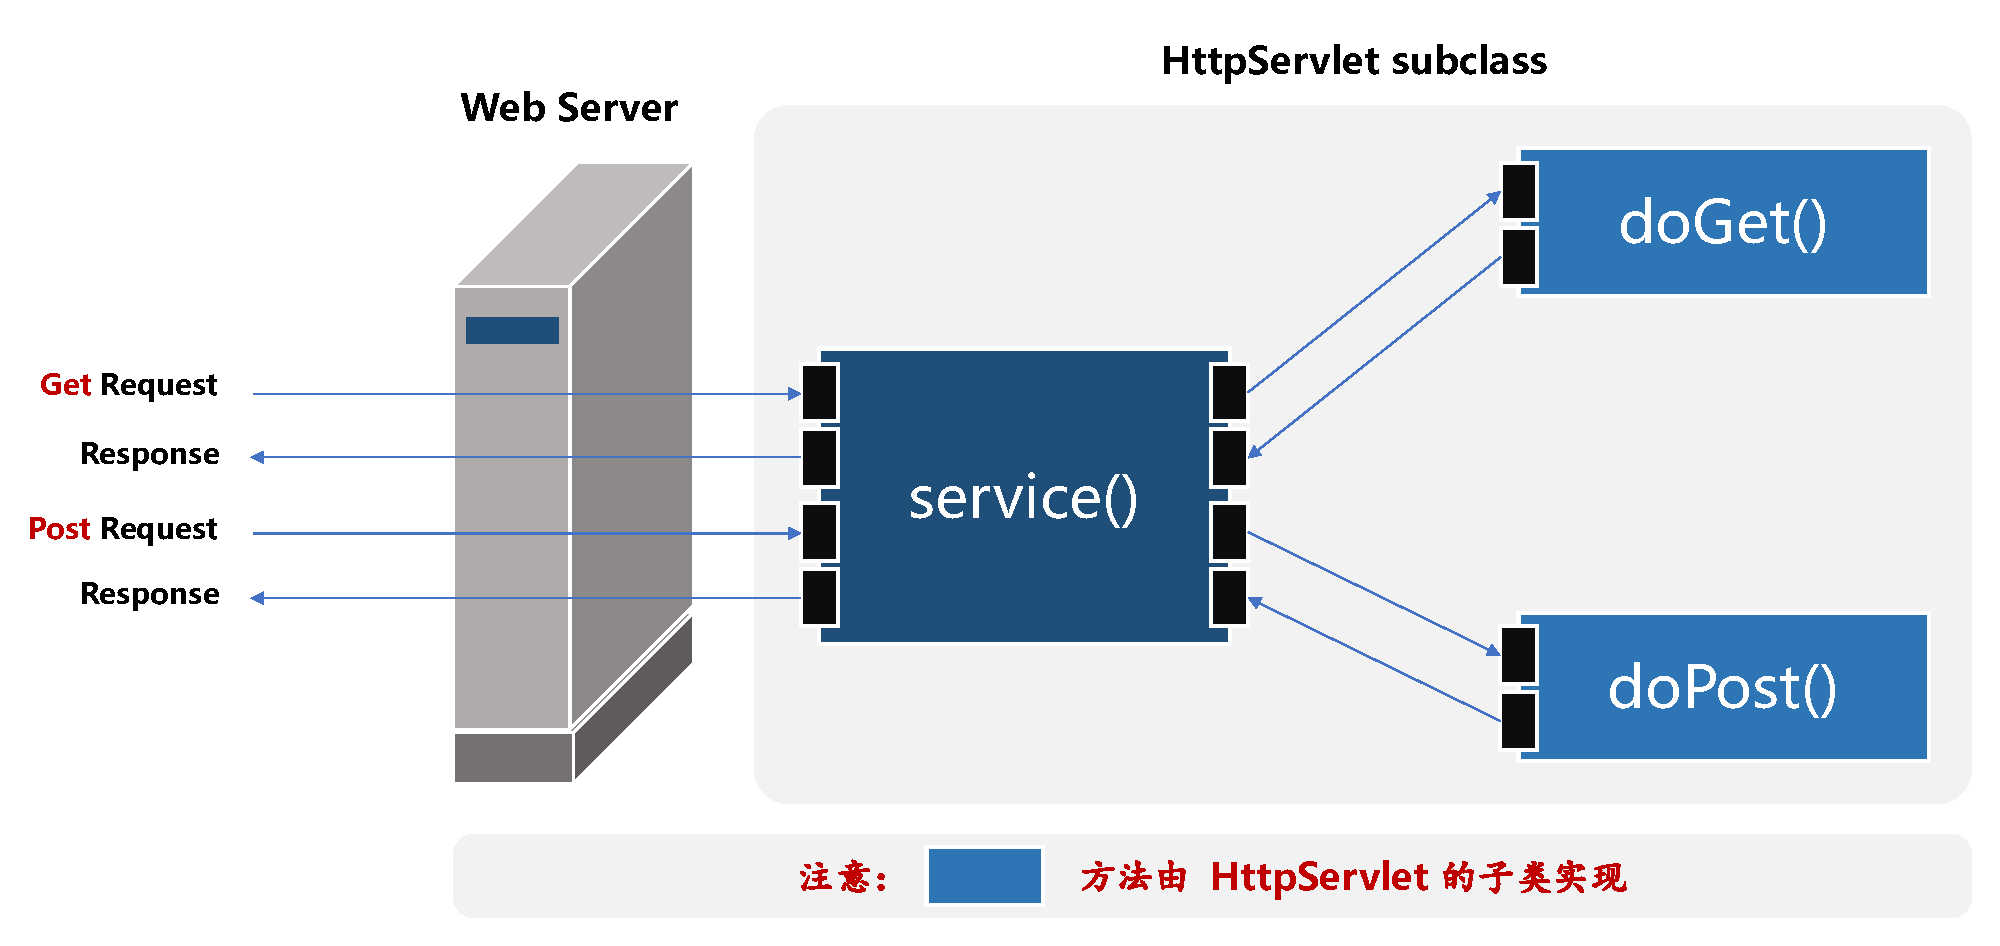
\includegraphics[width=0.8\textwidth]{images/JavaEE-servlet-programming/fig-servlet-mechanism.pdf}
\caption{Servlet处理流程}
\label{fig:servlet-mechanism}
\end{figure}


\section{Servlet配置}

\begin{itemize}
\item Servlet作为Web组件可以处理HTTP请求/响应,因此对外要求一个唯一的URL地址。
\item Servlet是一个Java类文件,不像JSP那样直接存放在Web目录下就能获得URL请求访问地址。
\item Servlet必须在Web的配置文件{\Red /WEB-INF/web.xml}中进行配置和映射才能响应HTTP请求。
\item Servlet的配置分为{\hei 声明和映射}两个步骤。
\end{itemize}

\subsection{Servlet声明}

通知Web容器Servlet的存在。

\begin{xmlCode}
  <servlet>
    <servlet-name>loginaction</servlet-name>
    <servlet-class>ouc.java.servlet.LoginAction</servlet-class>
  </servlet>  
\end{xmlCode}

\begin{description}
\item[<servlet-name>] 声明Servlet的名字,要求在一个web.xml文件内名字唯一。
\item[<servlet-class>] 指定Servlet的全名,即包名.类名。
\end{description}

\subsection{Servlet初始参数}

在Servlet的声明中可以配置Servlet初始参数,如数据库的Driver、URL、账号和
密码等信息。在Servlet中可以读取这些信息,避免在Servlet代码中定义这些信
息,修改时无需重新编译Servlet。

\begin{xmlCode}
  <servlet>
    <init-param>
      <param-name>driver</param-name>
      <param-value>sun.jdbc.odbc.JdbcOdbcDriver</param-value>
    </init-param>
  </servlet>
\end{xmlCode}

在Servlet中取得以上定义的参数的方法:

\begin{javaCode}
  String driver = config.getInitParameter("driver");
\end{javaCode}

\subsection{Servlet启动时机}

在配置Servlet时,可以指示Servlet跟随Web容器一起自动启动。这
时,Servlet就可以在没有请求的情形下,进行实例化和初始化,完成特定任务。
自启动Servlet的配置语法:

\begin{xmlCode}
  <load-on-startup>2</load-on-startup>
\end{xmlCode}

数字越小越先启动,0表示紧跟Web容器启动后第一个启动。


\subsection{Servlet映射}

\begin{itemize}
\item 任何Web文档在Internet上都要有一个URL地址才能被请求访问。
\item Servlet不能像JSP一样直接放在Web的发布目录上,需要单独映射URL地址。
\item 在{\Red /WEB-INF/web.xml}中进行Servlet的URL映射。
\end{itemize}

\tta{映射语法}

\begin{xmlCode}
  <servlet-mapping>
    <servlet-name>servlet name</servlet-name>
    <url-pattern>URL</url-pattern>
  </servlet-mapping>
\end{xmlCode}

{\kai 其中,servlet name与Servlet声明中的名称要一致。}

\tta{映射地址方式 \ding{182} 绝对地址方式映射}

\begin{xmlCode}
  <servlet-mapping>
    <servlet-name>LoginAction</servlet-name>
    <url-pattern>/login.action</url-pattern>
  </servlet-mapping>
\end{xmlCode}

\tta{映射地址方式 \ding{183} 匹配目录模式映射方式}

\begin{xmlCode}
  <servlet-mapping>
    <servlet-name>MainAction</servlet-name>
    <url-pattern>/main/*</url-pattern>
  </servlet-mapping>
\end{xmlCode}

在这个配置中,只要以/main开头的任何URL都能请求此Servlet。

\tta{映射地址方式 \ding{184} 匹配扩展名模式映射方式}

\begin{xmlCode}
  <servlet-mapping>
    <servlet-name>MainAction</servlet-name>
    <url-pattern>*.action</url-pattern>
  </servlet-mapping>
\end{xmlCode}

以上配置中扩展名为action的任何请求均被此Servlet响应。

{\Red\kai 注意:不能混合使用以上两种配置模式,否则会在Web项目部署并运行时产生运行时错误。}

如以下配置是错误的:

\begin{xmlCode}
<servlet-mapping>
  <servlet-name>MainAction</servlet-name>
  <url-pattern>/main/*.action</url-pattern>
</servlet-mapping>
\end{xmlCode}

\section{Servlet部署}

编译好的Servlet class文件应该放到指定的Web应用目录下,才能被Web容器找到,
这个路径为:{\Red /WEB-INF/classes/package/FileName.class}

例如Servlet类LoginAction:

\begin{javaCode}
package ouc.java.servlet;
public class LoginAction extends HttpServlet {
  //     
}
\end{javaCode}

存放路径为:
{\Blue /WEB-INF/classes/ouc/java/servlet/LoginAction.class}

\section{Servlet示例} 

\subsection{Eclipse}

New Project \ding{223} Web \ding{223} Dynamic Web Project \ding{223} Next >

\begin{itemize}
\item Project name: {\Blue sample.servlet}
\item Target runtime: {\Blue Apache Tomcat v8.0}
\item Dynamic web module version: 3.0
\item Configuration: {\Blue Default Configuration for Apache Tomcat v8.0}
\end{itemize}

\ding{223} Next >

Source folder on build path: {\Blue src}

\ding{223} Next >

{\Blue\ding{52}} Generate web.xml deployment descriptor

\ding{223} Finish

\subsection{WebContent/WEB-INF/web.xml}

Add following statements between <web-app> and </web-app>.

\begin{xmlCode}
  <servlet>
    <servlet-name>HelloServlet</servlet-name>
    <servlet-class>ouc.javaweb.HelloServlet</servlet-class>
    <load-on-startup>0</load-on-startup>
  </servlet>
    
  <servlet-mapping>
    <servlet-name>HelloServlet</servlet-name>
    <url-pattern>/hello</url-pattern>
  </servlet-mapping>  
\end{xmlCode}

\subsection{Java Resources/src}

Create java class file named ``HelloServlet.java''.

\begin{javaCode}
  package ouc.javaweb;

  import java.io.IOException;
  import java.io.PrintWriter;
  import javax.servlet.ServletException;
  import javax.servlet.http.HttpServlet;
  import javax.servlet.http.HttpServletRequest;
  import javax.servlet.http.HttpServletResponse;

  public class HelloServlet extends HttpServlet {
    public void doGet(HttpServletRequest request, HttpServletResponse response)
    throws ServletException, IOException {
      response.setContentType("text/html");
      response.setCharacterEncoding("UTF-8");
      PrintWriter out = response.getWriter();
      out.println("<html>");
      out.println("<head><title>A Servlet Sample</title></head>");
      out.println("<body>");
      out.println("<h1>Hello, Servlet!</h1>");
      out.println("A Servlet is a Java-based server-side web technology. ");
      out.println("</body></html>"););
      out.flush();
      out.close();
    }
  }
\end{javaCode}

sample.servlet \ding{223} 鼠标右键 \ding{223} Run as \ding{223} Run on Server

 \ding{223} Choose an existing server \ding{223} Tomcat v8.0 Server at localhost \ding{223} Finish

在浏览器中请求页面{\Blue http://localhost:8080/sample.servlet/hello}。

\section{课后习题}

\tta{问答题}

\begin{enumerate}
\item Servlet和一般Java类的区别是什么?
\item 简述Servlet的生命周期。
\item 简述Servlet与URL地址的映射方式(包括web.xml配置和基于注解)。
\end{enumerate}

\tta{小编程}

\begin{enumerate}
\item 编写一个能够计数访问次数的Servlet,每次请求次数增加1,并显示当前总访问次数。
\end{enumerate}